%%%%%%%%%%%%%%%%%%%%%%%%%%%%%%%%%%%
% Basic formatting and settings
%%%%%%%%%%%%%%%%%%%%%%%%%%%%%%%%%%%
\documentclass[12pt,a4paper]{report}
\usepackage[utf8x]{inputenc}
\usepackage[IL2]{fontenc}
\usepackage{a4wide}
\usepackage[left=2cm, right=2cm, top=2.5cm, bottom=2.5cm]{geometry}

%%%%%%%%%%%%%%%%%%%%%%%%%%%%%%%%%%%
% Include required packages
%%%%%%%%%%%%%%%%%%%%%%%%%%%%%%%%%%%
\usepackage{amsmath,amssymb,amsthm}
\usepackage[usenames]{color}
\usepackage{nicefrac}
\usepackage{verbatim}
\usepackage{graphicx}
\usepackage{enumitem}
\usepackage{setspace}
\usepackage{tabularx}
\usepackage{listings}
\usepackage[section]{placeins}

\usepackage[pdftex,bookmarks=true,colorlinks,linkcolor=blue,urlcolor=blue,unicode]{hyperref}
\hypersetup{pdftitle=ODCleanStore}

%%%%%%%%%%%%%%%%%%%%%%%%%%%%%%%%%%%
% Additional formatting settings
%%%%%%%%%%%%%%%%%%%%%%%%%%%%%%%%%%%

%\pagestyle{plain}
\pagestyle{headings}
\linespread{1.1}
\setcounter{secnumdepth}{3}
\setcounter{tocdepth}{2}

%%%%%%%%%%%%%%%%%%%%%%%%%%%%%%%%%%%
% Include macro definitions and package settings
%%%%%%%%%%%%%%%%%%%%%%%%%%%%%%%%%%%

%%%%%%%%%%%%%%%%%%%%%%%%%%%%%%%%%%%
% Indent settings for paragraphs, itemize and enumerate environment
%%%%%%%%%%%%%%%%%%%%%%%%%%%%%%%%%%%
\setitemize{noitemsep,topsep=2pt,leftmargin=30pt}
\setenumerate{noitemsep,topsep=2pt,leftmargin=30pt}
\setdescription{style=sameline}
%\setlength{\parindent}{0pt} % nastavuje odsazení prvniho radku
%\setlength{\parskip}{1.2ex plus 0.5ex minus 0.2ex} % odstup mezi odstavci

\newcommand{\moreindent}{\addtolength{\leftskip}{1.8em}}
\newcommand{\lessindent}{\addtolength{\leftskip}{1.8em}}
\newcommand{\suppressgaps}{\setlength{\parskip}{0pt}}

%%%%%%%%%%%%%%%%%%%%%%%%%%%%%%%%%%%
% Shortcuts for math mode
%%%%%%%%%%%%%%%%%%%%%%%%%%%%%%%%%%%
\newcommand{\coloneqq}{\mathrel{\mathop:}=}
\renewcommand{\O}{{\mathcal{O}}}
\newcommand{\etc}[2]{#1_1,\ldots,#1_#2}
\def\<#1>{\leavevmode\hbox{\it #1\/}} % usage: \<variable>

%%%%%%%%%%%%%%%%%%%%%%%%%%%%%%%%%%%
% Other shortcuts and style commands
%%%%%%%%%%%%%%%%%%%%%%%%%%%%%%%%%%%
\newcommand{\quot}[1]{``#1''}
\newcommand{\code}[1]{\texttt{#1}}
\newcommand{\varcode}[1]{\textit{\textless #1\textgreater}}
\newcommand{\vartext}[1]{\textit{#1}}
\newcommand{\tab}{\rule{30pt}{0pt}}
\newcommand{\term}[1]{\textit{#1}}
\newcommand{\todo}[1]{}
\newcommand{\importantterm}[1]{\textbf{#1}}

% These macros use a dirty trick to persuade LaTeX to typeset chapter headers
% more readably and not to leave plenty of space above them.
\makeatletter
\def\@makechapterhead#1{
  {\parindent \z@ \raggedright \normalfont
   \Huge\bfseries \thechapter. #1
   \par\nobreak
   \vskip 20\p@
}}
\def\@makeschapterhead#1{
  {\parindent \z@ \raggedright \normalfont
   \Huge\bfseries #1
   \par\nobreak
   \vskip 20\p@
}}
\makeatother

% Chapter that is not numbered but included in the contents
\def\chapwithtoc#1{
\chapter*{#1}
\addcontentsline{toc}{chapter}{#1}
} 

\newenvironment{enumeratei}
	{
		\begin{enumerate}
		\renewcommand{\labelenumi}{(\textit{\roman{enumi}})}
	}
	{
		\end{enumerate}
	}

\newenvironment{glossarylist}
	{\begin{description}[style=nextline,itemsep=8pt]}
	{\end{description}}

\newenvironment{configlist}
	{\begin{description}[style=nextline,font=\ttfamily]}
	{\end{description}}

\newenvironment{dirlist}
	{\begin{description}[style=sameline,font=\ttfamily]}
	{\end{description}}
	
%%%%%%%%%%%%%%%%%%%%%%%%%%%%%%%%%%%
% Package settings
%%%%%%%%%%%%%%%%%%%%%%%%%%%%%%%%%%%%

% lstlistings environment
% Defines a custom trivlisting environment
\lstset{basicstyle=\ttfamily\footnotesize,columns=flexible,
  frame=lines,float=ht,captionpos=b,aboveskip=1.5\bigskipamount}
\lstnewenvironment{trivlisting}
  {\lstset{basicstyle=\ttfamily,aboveskip=\medskipamount,frame=none}}
  {}

%%%%%%%%%%%%%%%%%%%%%%%%%%%%%%%%%%%
% Document-specific commands
%%%%%%%%%%%%%%%%%%%%%%%%%%%%%%%%%%%
\newcommand{\refusermanual}{User Manual\xspace}
\newcommand{\refadminmanual}{Administrator's \& Installation Manual\xspace}
\newcommand{\refprogrammersguide}{Programmer's Guide\xspace}
\newcommand{\configdefault}[1]{\newline\textit{Default value:}~\code{#1}}
\newcommand{\odcs}{ODCleanStore\xspace}
\newcommand{\reqparagraph}[1]{\paragraph{\textnormal{\textit{#1}}}}

%%%%%%%%%%%%%%%%%%%%%%%%%%%%%%%%%%%
% Aligned enumeration tables
%%%%%%%%%%%%%%%%%%%%%%%%%%%%%%%%%%%
\newcommand{\enumtable}[1]
{
	\begin{table}[!ht]
		\begin{tabularx}{\linewidth}{>{\textbf\bgroup}l<{\egroup}X}
			#1
		\end{tabularx}
	\end{table}
}

%%%%%%%%%%%%%%%%%%%%%%%%%%%%%%%%%%%
% Aligned field description tables
%%%%%%%%%%%%%%%%%%%%%%%%%%%%%%%%%%%
\newcommand{\fieldtable}[1]
{
	\begin{table}[!ht]
		\begin{tabularx}{\linewidth}{|>{\textbf\bgroup}l<{\egroup}|p{3cm}|X|}
			\hline
			\textnormal{Required} & Field & Description \\
			\hline \hline
			#1 \\
			\hline
		\end{tabularx}
	\end{table}
}


%%%%%%%%%%%%%%%%%%%%%%%%%%%%%%%%%%%
% Optionally disable use of images.
% Convenient for export to .dvi when the documents contain images not supported in plain latex
% Uncomment to disable images.
%%%%%%%%%%%%%%%%%%%%%%%%%%%%%%%%%%%
%\renewcommand{\includegraphics}[2][1]{}

\newcommand{\version}{0.3.1}
\newcommand{\documentname}{\refadminmanual}

\hypersetup{pdftitle=ODCleanStore -- \documentname}

\begin{document}

\title{ODCleanStore -- \documentname}

\begin{titlepage}
\begin{center}

\large
Charles University in Prague

\smallskip

Faculty of Mathematics and Physics

%\vspace{\stretch{1}}
%{\bf\Large SOFTWARE PROJECT}

\vspace{\stretch{3}}

\resizebox{0.5\linewidth}{!}{\bf\Huge ODCleanStore}

%\bigskip
%\resizebox{0.3\linewidth}{!}{Open Data store}

\vspace{\stretch{3}}
\begin{spacing}{1.5} 
{\bf\Huge \documentname}
\end{spacing}

\vspace{\stretch{1}}
Release \version\\
\today

\vspace{\stretch{15}}

\begin{tabular}{rl}

\textbf{Authors:} & Jan Michelfeit \\
& Du\v san Rychnovsk\'y\\
& Jakub Daniel\\
& Petr Jerman\\
& Tom\' a\v s Soukup\\
\noalign{\vspace{3mm}}
\textbf{Supervisor:} & RNDr. Tom\' a\v s Knap
\end{tabular}

\end{center}
\end{titlepage}

\newpage

\renewcommand{\contentsname}{Contents}
\tableofcontents
\bigskip

\newpage

%%%%%%%%%%%%%%%%%%%%%%%%%%%%%%%%%%%%%%%%%%%%%%%%%%%%%%%%%%%%%%%%%%%%%%%%%%%%%%

\chapter{Introduction}
\odcs is a~server application for management of Linked Data. It stores data in RDF, processes them and provides integrated views on the data.

This document serves as the installation guide and manual for system administrators. It includes system requirements, installation instructions, configuration overview, manual how to start the application and basic information about extending ODCleanStore's data processing capabilities by adding \term{custom transformers}.

\section*{What is ODCleanStore}
\odcs accepts arbitrary RDF data and metadata through a SOAP webservice (\term{Input Webservice}). The data is processed by \term{transformers} in one of a~set of customizable \term{pipelines} and stored to a~persistent store (OpenLink Virtuoso database instance). The stored data can be accessed again either  directly through a SPARQL endpoint or through \term{Output Webservice}. Linked Data consumers can send queries and custom query policies to Output Webservice and receive (aggregated/integrated) RDF data relevant for their query, together with information about provenance and data quality. 

\section*{Related documents}
More detailed information about \odcs from the perspective of a user can be found in related document \quot{\refusermanual}. It also contains definition of user roles, glossary of terms etc. Document \quot{\refprogrammersguide} contains more detailed information intended primarily for developers, system administrators, however, may also find interesting in-depth information in \refprogrammersguide. 


\chapter{System Requirements}
\label{chap:requirements}
\odcs is a multiplatform application written in Java. These are the system requirements for installing and running \odcs:

\begin{itemize}
  \item Operating System: Windows XP, Windows 7, Windows Server 2008, Linux
  \item Java Runtime Environment 6 or newer\footnote{\url{http://www.java.com/en/download/}}
  \item Installed OpenLink Virtuoso\footnote{\url{http://virtuoso.openlinksw.com/}} (see below)
  \item Apache Tomcat\footnote{\url{http://tomcat.apache.org/}} (or an equivalent Java servlet container)
\end{itemize}


\section{OpenLink Virtuoso}
\label{sec:virtuoso}
\odcs uses two instances of Virtuoso database for storing data -- one is used for storing data that are currently being processed (\term{dirty database instance}) and the other for already processed data visible to end users (\term{clean database instance}). 

\odcs requires that the two instances of Virtuoso database are created before the installation process. If you are familiar with Virtuoso and already have two Virtuoso instances that you would like to use, you can skip the rest of this section -- make sure, however, to modify \odcs configuration options accordingly  (see Chapter \ref{chap:configOptions}). In particular, set correct database settings and include a directory specified in \code{engine.clean\_import\_export\_dir} and \code{engine.dirty\_import\_export\_dir} configuration options in \code{DirsAllowed} option of Virtuoso configuration.

\subsection{Creating Database Instances}
Virtuoso has a paid enterprise license, but also an open source edition\footnote{\url{http://virtuoso.openlinksw.com/dataspace/dav/wiki/Main/VOSDownload}} available for free. In order to install it, follow instructions on the download page. Make sure that the deployed binaries (\varcode{installation-directory}/bin) are on your system PATH (you can test it by running commands \code{isql} and \code{virtuoso-t}).

\odcs distribution contains files \code{virtuoso.ini-clean} and \code{virtuoso.ini-dirty}. While it is not required, we strongly recommend creating the two database instances with these provided configuration files.

\begin{enumerate}
  \item \label{itm:dbInstDirs} Create one empty directory for each database instance.
  \item \label{itm:dbInstCleanStart} Copy \code{virtuoso.ini-clean} to the directory for the clean database instance, create a copy of the file and name it \code{virtuoso.ini}. If you are familiar with Virtuoso, you may customize configuration in \code{virtuoso.ini} according to your needs. 
  \item Create a new database instance by executing
\begin{verbatim}
  virtuoso-t +service create +instance odcsclean +configfile virtuoso.ini
\end{verbatim}
    in the directory for the clean database instance.
    \item \label{itm:dbInstCleanEnd} Start the newly creted database instance by executing
\begin{verbatim}
  virtuoso-t +service start +instance odcsclean
\end{verbatim}
  
  \item Copy \code{virtuoso.ini-dirty} to the directory for the dirty database instance created in step \ref{itm:dbInstDirs}. Create a copy of the file and name it \code{virtuoso.ini}. If you are familiar with Virtuoso, you may customize configuration in \code{virtuoso.ini} according to your needs. 
  \item Create a new database instance by executing
\begin{verbatim}
  virtuoso-t +service create +instance odcsdirty +configfile virtuoso.ini
\end{verbatim}
    in the directory for the dirty database instance.
    \item  Start the newly creted database instance by executing
\begin{verbatim}
  virtuoso-t +service start +instance odcsdirty
\end{verbatim}
\end{enumerate}


\textit{Note:} For security reasons, don't forget to change credentials for your database instance.


\chapter{Installation CD Contents}
This chapter describes the contents of the installation CD with \odcs:
%TODO

\begin{description}[style=nextline,font=\ttfamily]
  \item[engine/] Contains binaries of \odcs Engine.
  \item[odcs-installer.sh] Installation script for Linux.
  \item[odcs-installer.bat] Installation script for Windows.
  \item[odcs-installer.jar] Binary with the \odcs installer.
  \item[clean-clear.sql] SQL script for clearing the clean database instance.
  \item[clean-fulltext-index.sql] SQL script for creating a fulltext index on the clean database instance. Required for working keyword queries.
  \item[clean.sql] SQL script for importing initial data to the clean database instance.
  \item[dirty-clear.sql] SQL script for clearing the dirty database instance.
  \item[dirty.sql] SQL script for importing initial data to the dirty database instance.
  \item[odcs-webfrontend.war] Java web application archive containing Administration Frontend of \odcs.
\end{description}

\chapter{Step by Step Installation Guide}
\odcs can be installed with a provided installer with graphical interface.
%Alternatively, \odcs can be installed manually following instructions in the README file.

\section{Prerequisities}
Before installation, make sure your system satisfies requirements listed in Chapter \ref{chap:requirements}. In particular, make sure to have two Virtuoso database instances created and \textit{started} before installation, as described in Section \ref{sec:virtuoso}.

\section{Using the Installer}
In order to run the installer, execute in the root directory of the distribution
\begin{verbatim}
  ./odcs-installer.sh
\end{verbatim}
on Linux, or run
\begin{verbatim}
  odcs-installer.bat
\end{verbatim}
on Windows. This should start the installer.

On the first screen of the installer, enter the directory where \odcs binaries should be installed.

\begin{figure}[!h]
    \centering
    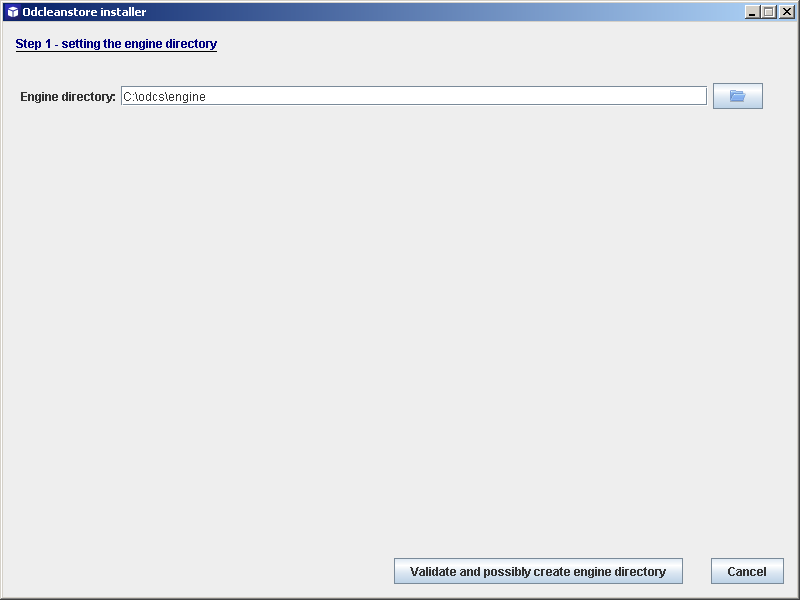
\includegraphics[width=0.8\textwidth]{images/install-step01.png}
    %\caption{}
    %\label{fig:}
\end{figure}

\FloatBarrier

%TODO
On the second screen, you can see the progress of copying files to the installation directory.

\begin{figure}[!h]
    \centering
    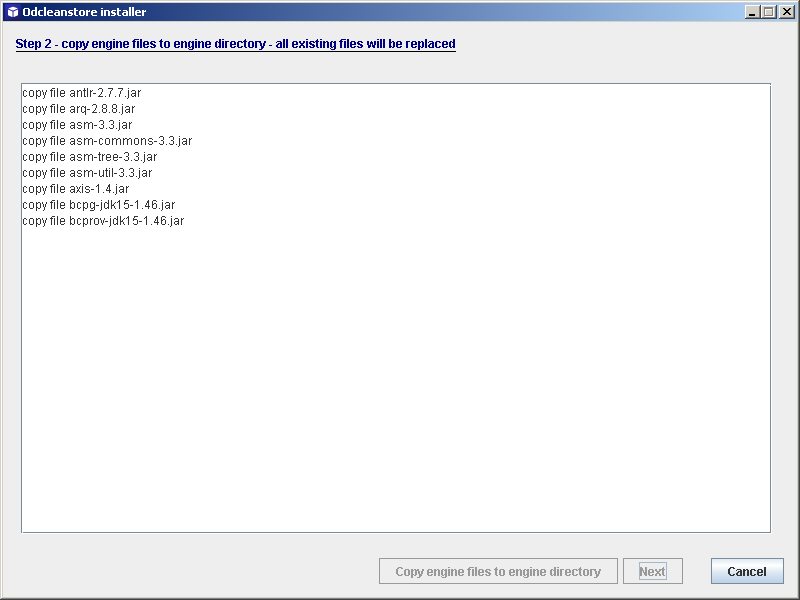
\includegraphics[width=0.8\textwidth]{images/install-step02.png}
    %\caption{}
    %\label{fig:}
\end{figure}

\FloatBarrier

Next, enter the connection settings for the clean and dirty Virtuoso database instances. See Section \ref{sec:virtuoso} for more information about Virtuoso database instances.

\begin{figure}[!h]
    \centering
    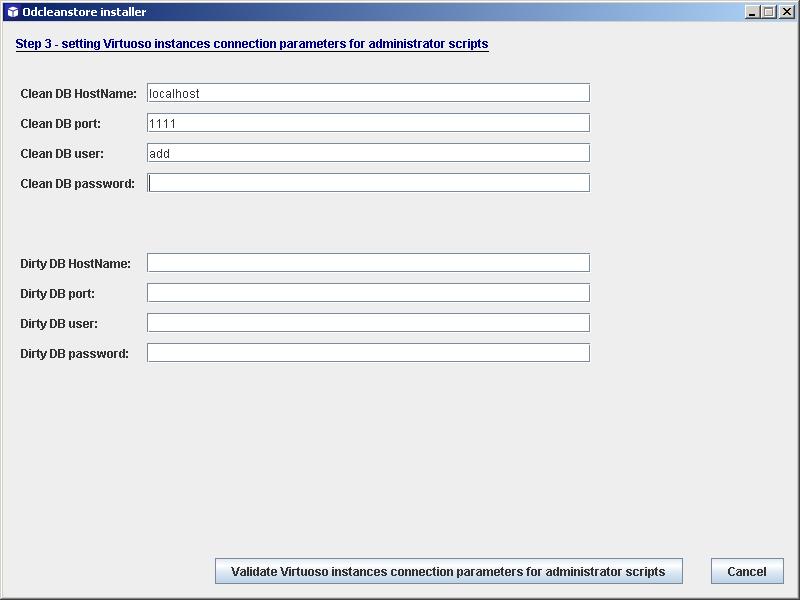
\includegraphics[width=0.8\textwidth]{images/install-step03.png}
    %\caption{}
    %\label{fig:}
\end{figure}

\FloatBarrier

The next screen shows the progress of database import.

\begin{figure}[!h]
    \centering
    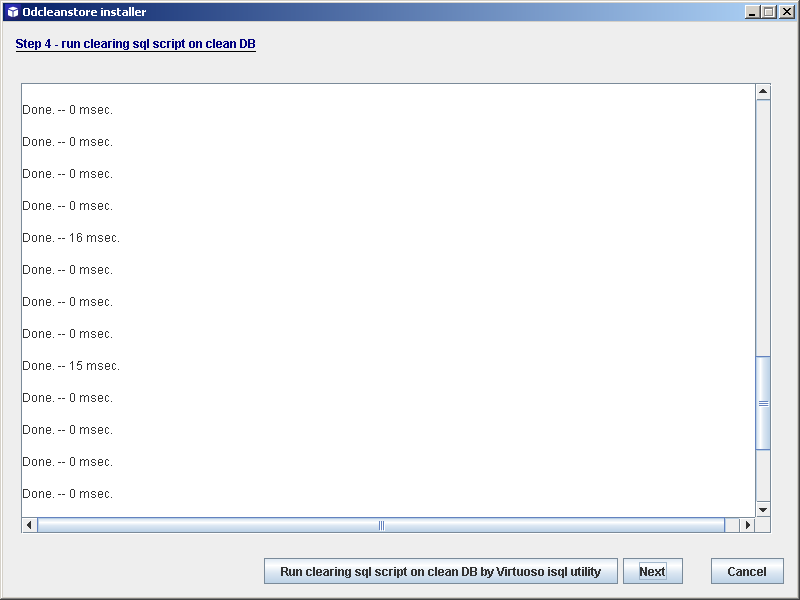
\includegraphics[width=0.8\textwidth]{images/install-step04.png}
    %\caption{}
    %\label{fig:}
\end{figure}

\FloatBarrier

\begin{figure}[!h]
    \centering
    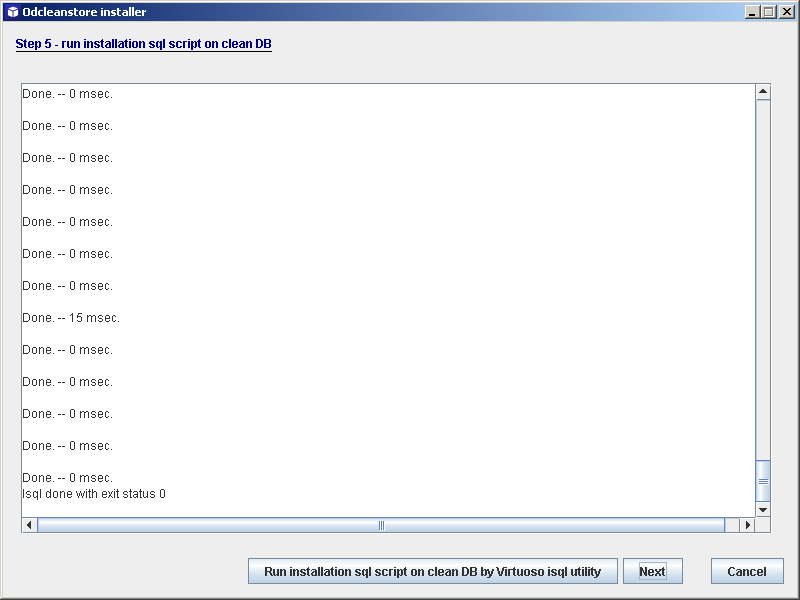
\includegraphics[width=0.8\textwidth]{images/install-step05.png}
    %\caption{}
    %\label{fig:}
\end{figure}

\FloatBarrier

\begin{figure}[!h]
    \centering
    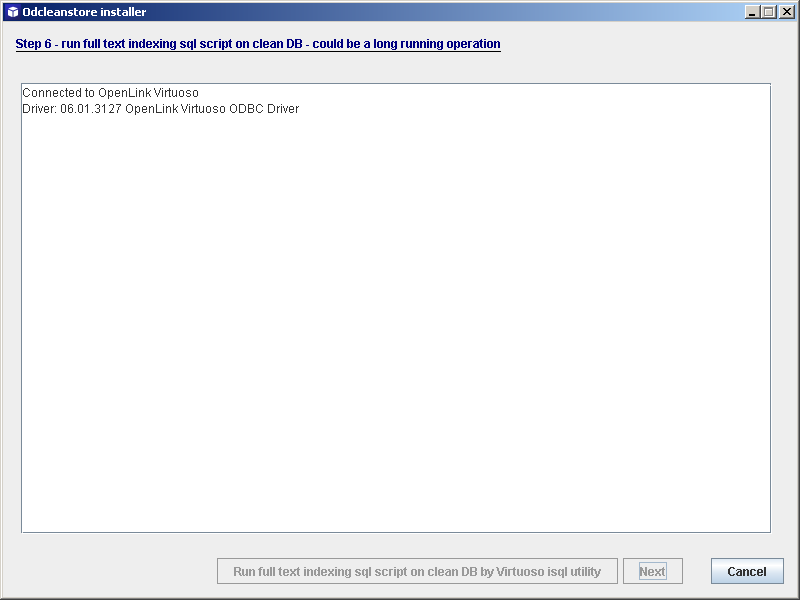
\includegraphics[width=0.8\textwidth]{images/install-step06.png}
    %\caption{}
    %\label{fig:}
\end{figure}

\FloatBarrier

\begin{figure}[!h]
    \centering
    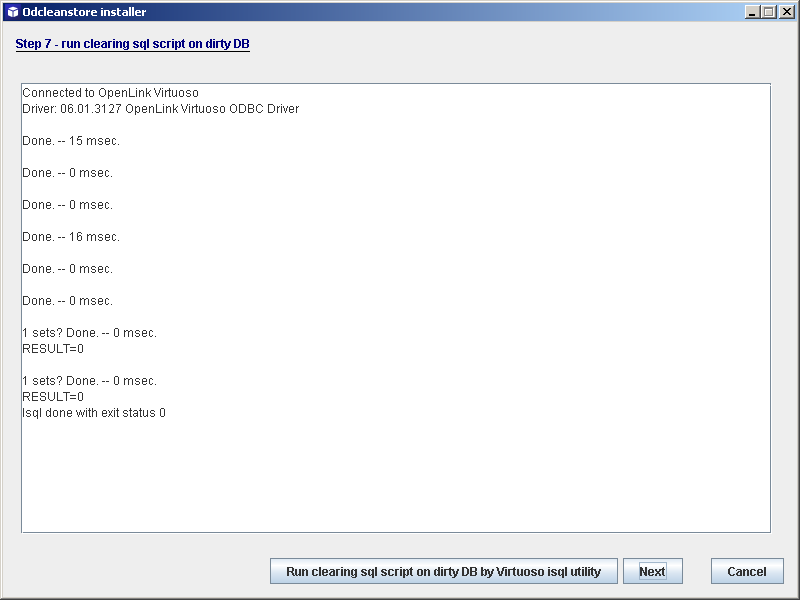
\includegraphics[width=0.8\textwidth]{images/install-step07.png}
    %\caption{}
    %\label{fig:}
\end{figure}

\FloatBarrier

\begin{figure}[!h]
    \centering
    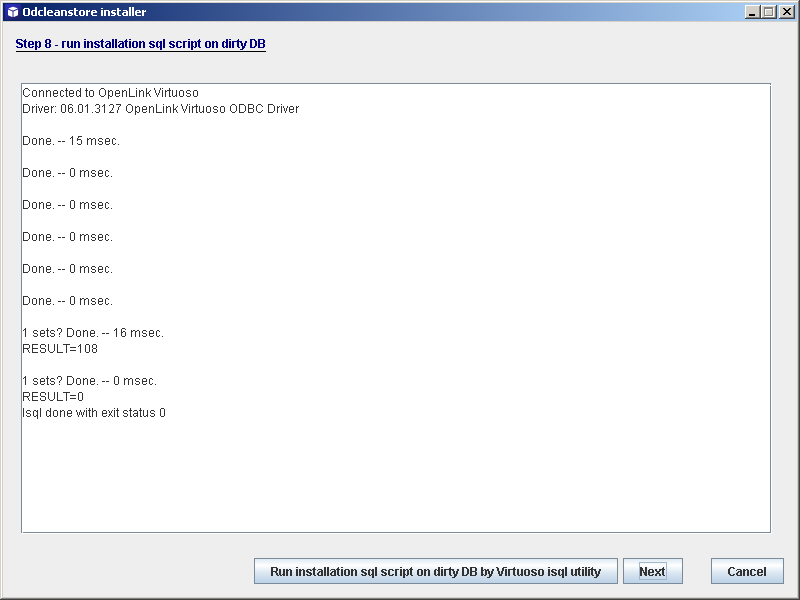
\includegraphics[width=0.8\textwidth]{images/install-step08.png}
    %\caption{}
    %\label{fig:}
\end{figure}

\FloatBarrier

\begin{figure}[!h]
    \centering
    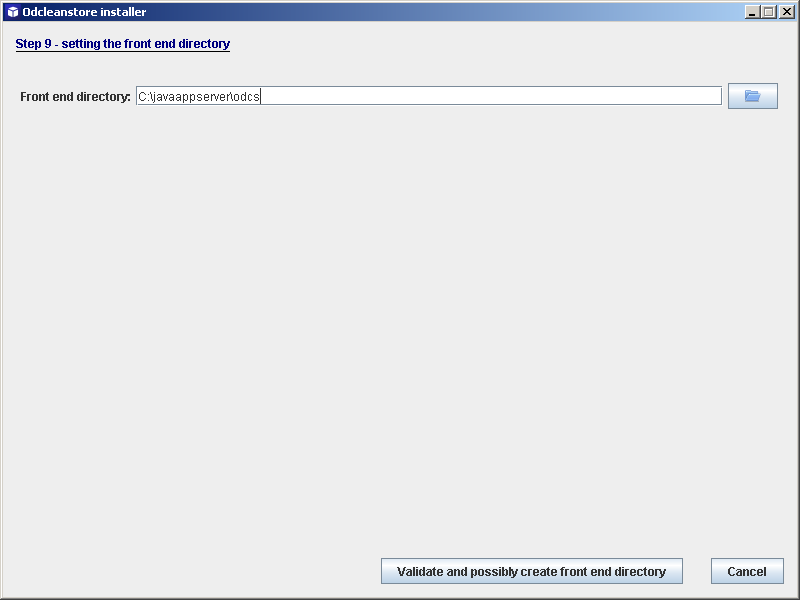
\includegraphics[width=0.8\textwidth]{images/install-step09.png}
    %\caption{}
    %\label{fig:}
\end{figure}

\FloatBarrier

\begin{figure}[!h]
    \centering
    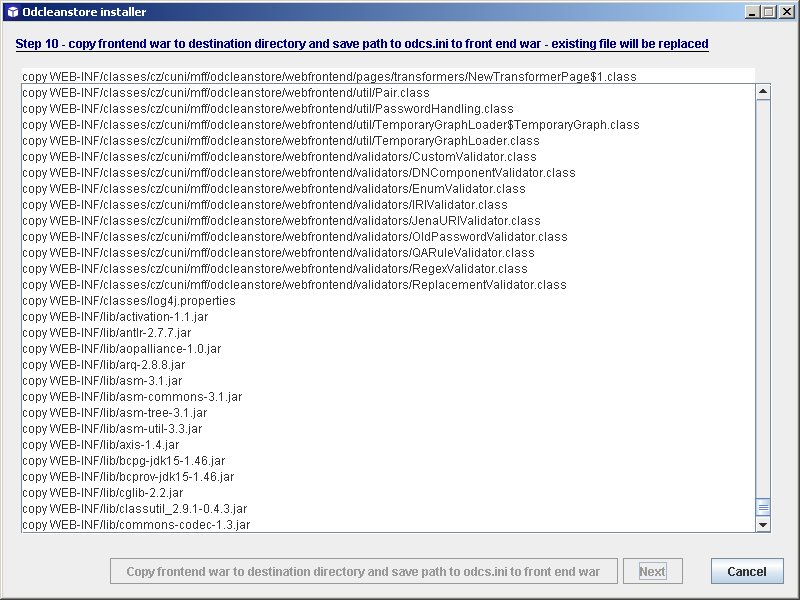
\includegraphics[width=0.8\textwidth]{images/install-step10.png}
    %\caption{}
    %\label{fig:}
\end{figure}

\FloatBarrier

\begin{figure}[!h]
    \centering
    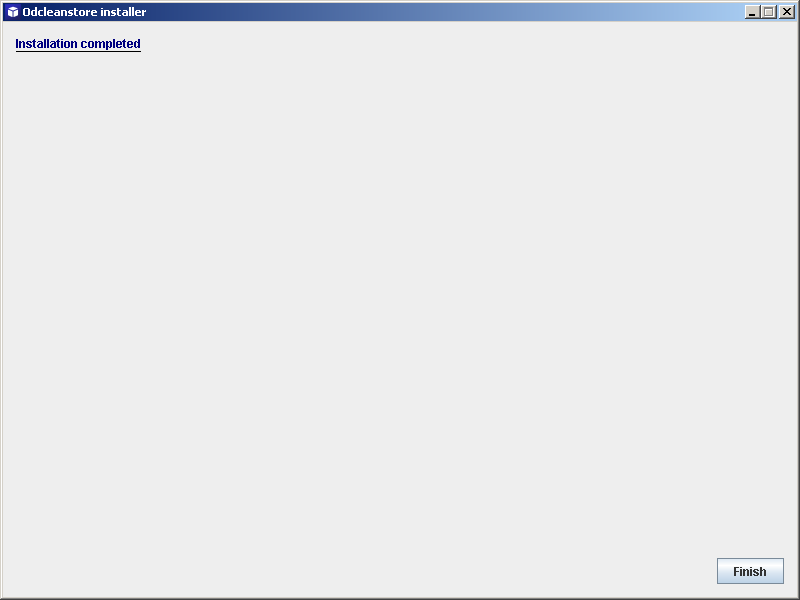
\includegraphics[width=0.8\textwidth]{images/install-step11.png}
    %\caption{}
    %\label{fig:}
\end{figure}

\FloatBarrier

\section{Post-installation Steps}
After successfull install, you may customize default \odcs settings in the configuration file \code{odcs.ini} in the Engine installation directory. See Chapter \ref{chap:configOptions} for description of all options.

The installer deploys the web archive with \FE to the designated directory in your servlet container. Depending on the configuration of your servlet container, you may need to add the \FE web application to its configuration explicitly. If that is the case, in Tomcat, for example, this can be accomplished by adding a line similar to the following to <Host> section of Tomcat's \code{server.xml}:  
\begin{verbatim} 
    <Context path="" docBase="{path to odcs-webfrontend-<version>.war}"></Context>
\end{verbatim} 

%\chapter{(Contents of the Deployed Application)}

\chapter{Configuration Options}
 \label{chap:configOptions}
Global configuration options for ODCleanStore are stored in configuration file \code{odcs.ini} in the Engine installation directory.

The configuration file is used both by ODCleanStore Engine and administration frontend. Configuration options are loaded only once when the Engine or administration frontend is started, therefore, it is necessary to restart the Engine or administration frontend web application for the changes to take effect.
\todo{how to restart engine and webfrontend}

List with a description of all configuration options follows:

\subsection*{Database Configuration}
\begin{configlist}
	\item[db.clean.jdbc.connection\_string]
	  Connection string for JDBC access to the Virtuoso instance representing the clean database. Must contain connection charset.
		\configdefault{jdbc:virtuoso://localhost:1111/CHARSET=UTF-8}
	\item[db.clean.jdbc.username]
	  Username for JDBC access to the Virtuoso instance representing the clean database.
		\configdefault{dba}
	\item[db.clean.jdbc.password]
	  Password for JDBC access to the Virtuoso instance representing the clean database.
		\configdefault{dba}
	\item[db.clean.sparql.endpoint\_url]
	  URL of the SPARQL endpoint of the clean database. Used by Linker to read RDF data.
		\configdefault{http://localhost:8890/sparql}

	\item[db.dirty.jdbc.connection\_string]
		Connection string for JDBC access to the Virtuoso instance representing the dirty database. Must contain connection charset.
		\configdefault{jdbc:virtuoso://localhost:1112/CHARSET=UTF-8}
	\item[db.dirty.jdbc.username]
		Username for JDBC access to the Virtuoso instance representing the dirty database.
		\configdefault{dba}
	\item[db.dirty.jdbc.password]
		Password for JDBC access to the Virtuoso instance representing the dirty database.
		
	\item[db.dirty.sparql.endpoint\_url]
		URL of the SPARQL endpoint of the dirty database. Used by Linker to read RDF data.
		\configdefault{http://localhost:8891/sparql}
	\item[db.dirty\_update.sparql.endpoint\_url]
		URL of the secured SPARQL endpoint of the dirty database. Used by Linker to store created links.
		\configdefault{http://localhost:8891/sparql-auth}
	\item[db.dirty\_update.sparql.endpoint\_username]
		Name of the user, who is authorized for using SPARQL UPDATE on the authorized endpoint.
		\configdefault{SILK}
	\item[db.dirty\_update.sparql.endpoint\_password]
		Password of the user, who is authorized for using SPARQL UPDATE on the authorized endpoint.
		\configdefault{odcs}
\end{configlist}

\subsection*{Input Webservice Configuration}
\begin{configlist}
	\item[input\_ws.endpoint\_url]
		URL where the input webservice is listening.
		\configdefault{http://localhost:8088/inputws}
	\item[input\_ws.recovery\_crash\_penalty]
		Waiting penalty after Input Webservice recovery crash before recovery restart in milliseconds.
		\configdefault{60000}
	\item[input\_ws.named\_graphs\_prefix]
		Prefix of named graphs incoming where data \& metadata are stored. Must be a valid URL.
		\configdefault{http://opendata.cz/infrastructure/odcleanstore/}
\end{configlist}

\subsection*{Output Webservice Configuration}
\begin{configlist}
	\item[output\_ws.result\_data\_prefix]
		Prefix of named graphs and URIs where query results and metadata in the output are placed.
		\configdefault{http://opendata.cz/infrastructure/odcleanstore/query/}
	\item[output\_ws.port]
		Port of the output webservice
		\configdefault{8087}
	\item[output\_ws.keyword\_path]
		Relative path fragment for the keyword query over the output webservice.
		\configdefault{keyword}
	\item[output\_ws.uri\_path]
		Relative path fragment for the uri query over the output webservice.
		\configdefault{uri}
	\item[output\_ws.metadata\_path]
		Relative path fragment for the metadata query over the output webservice.
		\configdefault{metadata}
	\item[output\_ws.named\_graph\_path]
		Relative path fragment for the named graph query over the output webservice.
		\configdefault{namedGraph}
\end{configlist}

\subsection*{Query Execution Configuration}	
\begin{configlist}
	\item[query\_execution.max\_query\_result\_size]
		Maximum number of results allowed in each database query performed during a query execution. This option effectively affects the maximum number of results returned in response to a query through Ouptut Webservice to a multiple of this number (cca 3 times the value of this option).
		\configdefault{500}
\end{configlist}

\subsection*{Conflict Resolution Configuration}
\begin{configlist}
	\item[conflict\_resolution.agree\_coefficient]
		Agree coefficient used in aggregated quality formula -- value $N$ means that agreement of $N+1$ sources with score 1 on the same value will increase the quality of that value to 1.
			\configdefault{4}
	\item[conflict\_resolution.score\_if\_unknown]
			Graph score used if none is given in the input of Conflict Resolution (e.g. is unknown).
			\configdefault{1}
	\item[conflict\_resolution.named\_graph\_score\_weight]
			Weight of the named graph score in aggregated quality calculation (see \linebreak \code{conflict\_resolution.publisher\_score\_weight})
			\configdefault{0.8}
	\item[conflict\_resolution.publisher\_score\_weight]
			Weight of the graph publisher's score in aggregated quality calculation (see \linebreak \code{conflict\_resolution.named\_graph\_score\_weight})
			\configdefault{0.2}
	\item[conflict\_resolution.max\_date\_difference]
			Difference between two dates when their distance is equal to MAX\_DISTANCE constant, given in seconds. When the difference of two dates is higher or equal to this value, in Conflict Resolution, they are considered to be totally different; when the difference is smaller, the difference coefficient is proportionally smaller.
			\configdefault{31622400} (366 days)
\end{configlist}

\subsection*{Transformers Configuration}
\begin{configlist}
	\item[object\_identification.link\_within\_graph]
		Sets whether to link incoming data against itself by default.
		\configdefault{true}
	\item[object\_identification.link\_attachd\_graphs]
		Sets whether to link data from attached graphs created by preceding transformers by default.
		\configdefault{true}
\end{configlist}

\subsection*{Engine \& Backend Configuration}
\begin{configlist}
	\item[backend.query\_timeout]
		Timeout for database queries executed by predefined transformers, Query Execution and Engine in seconds.
		\configdefault{30}

	\item[engine.clean\_import\_export\_dir]
		Directory for Clean Virtuoso instance data import and export files. Base for relative path is clean db server root (directory of the Virtuoso INI file). Path or his parent must be specified in the DirsAllowed param in the virtuoso INI file and the Virtuoso server restarted for access to be allowed to the files by Virtuoso.
		\configdefault{odcs/}
		
	\item[engine.dirty\_import\_export\_dir]
		Directory for Dirty Virtuoso instance data import and export files. Base for relative path is clean db server root (directory of the Virtuoso INI file). Path or his parent must be specified in the DirsAllowed param in the virtuoso INI file and the Virtuoso server restarted for access to be allowed to the files by Virtuoso.  
		\configdefault{odcs/}
		
	\item[engine.startup\_timeout]
		Maximum time in milliseconds for services initializing before engine shutdown.
		\configdefault{30000}
		
	\item[engine.shutdown\_timeout]
		Maximum time in milliseconds for services shutdown before engine exit.
		\configdefault{30000}
	
	\item[engine.look\_for\_graph\_interval]
		Additional timer setting interval for lookup for graph for processing in milliseconds.
		\configdefault{8000}
		
	\item[engine.second\_crash\_penalty]
		Waiting penalty after double pipeline crash before pipeline restart in milliseconds
		\configdefault{60000}
		
	\item[engine.state\_to\_db\_writing\_interval]
		Interval for writing engine state information to db in milliseconds.
		\configdefault{5000}
	
	\item[engine.engine\_uuid]
		\configdefault{88888888-8888-8888-8888-888888888888}
\end{configlist}

\subsection*{Administration Frontend Configuration}
\begin{configlist}
	
	\item[web\_frontend.gmail\_address]
		Username of a GMAIL accout to send emails through.
		\configdefault{odcleanstore@gmail.com}
		
	\item[web\_frontend.gmail\_password]
		Password of a GMAIL accout to send emails through.
		\configdefault{odcleanstore2012}
		
	\item[web\_frontend.output\_ws\_host]
		Output webservice host.
		\configdefault{http://localhost}
		
	\item[web\_frontend.debug\_directory\_path]
		Path to transformer directory for debugging.
		\configdefault{./odcs-debug}
\end{configlist}


\chapter{Starting and Stopping the Application}
\section{Engine}
\odcs Engine can be started by executing the \code{run-engine.cmd} script (on Windows) or \code{run-engine.sh} script (on Unix) in the installation directory of \odcs Engine. The Engine will load its configuration from the \code{odcs.ini} file in this directory and, after initialization, automatically start listening on Input and Output Webservice ports for requests.

In order to stop Engine, simply press \code{Ctrl}+\code{C} in the console window with Engine (send SIGINT signal to the Engine process on Linux). Engine will shutdown all services, wait (up until a timeout) until the currently active pipeline transformer finishes, and stop.

Engine is also prepared to be run as a system service on Windows, or daemon on Linux, respectively. Installing \odcs as a service/daemon will be added to the installer in future.

\section{\FE}
\FE is a standard Java web application and its lifecycle depends on its servlet container -- please refer to documentation of your server container\footnote{E.g. \url{http://tomcat.apache.org/tomcat-7.0-doc/index.html}}. Usually, \FE would be reached by navigating to \code{http://localhost:8080/} in your web browser.

\chapter{Custom Transformers}
\label{chap:customTransformers}
The administrator may extend data-processing capabilities of \odcs by adding new custom transformers. In order to start using the transformer:
\begin{enumerate}
  \item Implement your custom transformer by implementing the \code{Transformer} interface in Java or other compatible language.\\
  The classfile for the \code{Transformer} interface is in \code{odcs-core-<version>.jar} file in the \odcs distribution, or can be obtained from sources in \code{odcs-core} maven artifact -- see chapter \quot{Setting up Development Environment} in \refprogrammersguide. \\
  For more information about how to implement a custom transformer and what features it should have, please refer to chapter \quot{Transformers – Introduction} in \refprogrammersguide.
  \item Save the .jar file with the implementation to a location where Engine can read it from the filesystem. The classfiles of the \code{odcs-core} maven artifact need not be included in the .jar file (as they will be already loaded by Engine when the custom transformer is loaded at runtime).
  \item In \FE, go to \quot{Transformers}~\textgreater~\quot{Add a new transformer} (\figurename~\ref{fig:customTransformer}). Enter the path to the .jar file with the implementation, the fully qualified name of the your class that implements the \code{Transformer} interface and fill in the other fields. Submit the form.
  \item Now, the custom transformer is registered and can be assigned to pipelines and used for data processing.
\end{enumerate}

\begin{figure}[h]
    \centering
    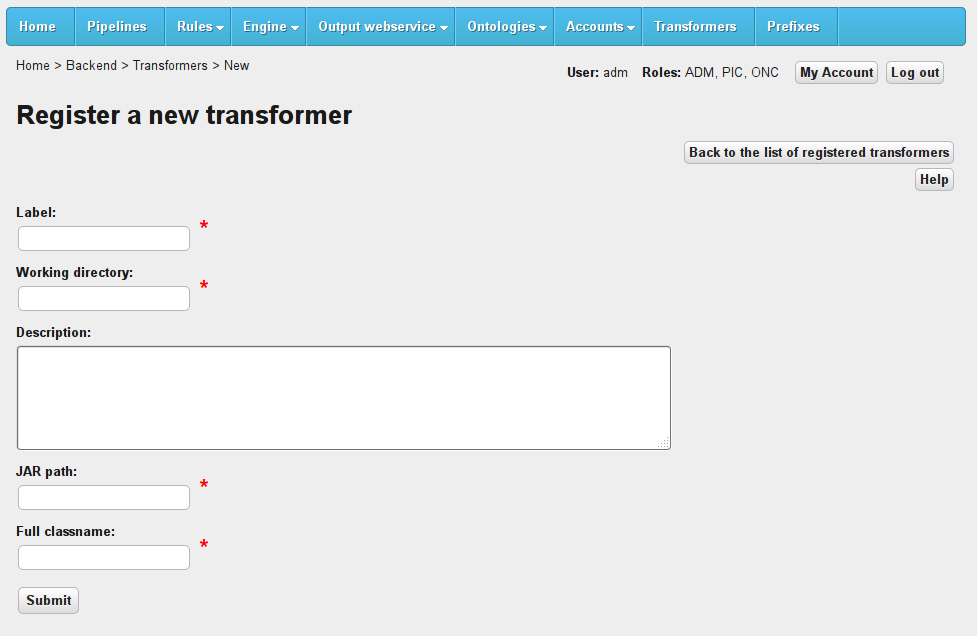
\includegraphics[width=0.7\textwidth]{images/fe-custom-transformer.png}
    \caption{Screen for registering a custom transformer}
    \label{fig:customTransformer}
\end{figure}


%\chapter{(Troubleshooting)}
% TODO based on real-world problems

%%%%%%%%%%%%%%%%%%%%%%%%%%%%%%%%%%%%%%%%%%%%%%%%%%%%%%%%%%%%%%%%%%%%%%%%%%%%%%

\appendix

\chapter{License}
ODCleanStore is released as open source software under Apache License, Version 2.0.

\begin{verbatim}
                                 Apache License
                           Version 2.0, January 2004
                        http://www.apache.org/licenses/

   TERMS AND CONDITIONS FOR USE, REPRODUCTION, AND DISTRIBUTION

   1. Definitions.

      "License" shall mean the terms and conditions for use, reproduction,
      and distribution as defined by Sections 1 through 9 of this document.

      "Licensor" shall mean the copyright owner or entity authorized by
      the copyright owner that is granting the License.

      "Legal Entity" shall mean the union of the acting entity and all
      other entities that control, are controlled by, or are under common
      control with that entity. For the purposes of this definition,
      "control" means (i) the power, direct or indirect, to cause the
      direction or management of such entity, whether by contract or
      otherwise, or (ii) ownership of fifty percent (50%) or more of the
      outstanding shares, or (iii) beneficial ownership of such entity.

      "You" (or "Your") shall mean an individual or Legal Entity
      exercising permissions granted by this License.

      "Source" form shall mean the preferred form for making modifications,
      including but not limited to software source code, documentation
      source, and configuration files.

      "Object" form shall mean any form resulting from mechanical
      transformation or translation of a Source form, including but
      not limited to compiled object code, generated documentation,
      and conversions to other media types.

      "Work" shall mean the work of authorship, whether in Source or
      Object form, made available under the License, as indicated by a
      copyright notice that is included in or attached to the work
      (an example is provided in the Appendix below).

      "Derivative Works" shall mean any work, whether in Source or Object
      form, that is based on (or derived from) the Work and for which the
      editorial revisions, annotations, elaborations, or other modifications
      represent, as a whole, an original work of authorship. For the purposes
      of this License, Derivative Works shall not include works that remain
      separable from, or merely link (or bind by name) to the interfaces of,
      the Work and Derivative Works thereof.

      "Contribution" shall mean any work of authorship, including
      the original version of the Work and any modifications or additions
      to that Work or Derivative Works thereof, that is intentionally
      submitted to Licensor for inclusion in the Work by the copyright owner
      or by an individual or Legal Entity authorized to submit on behalf of
      the copyright owner. For the purposes of this definition, "submitted"
      means any form of electronic, verbal, or written communication sent
      to the Licensor or its representatives, including but not limited to
      communication on electronic mailing lists, source code control systems,
      and issue tracking systems that are managed by, or on behalf of, the
      Licensor for the purpose of discussing and improving the Work, but
      excluding communication that is conspicuously marked or otherwise
      designated in writing by the copyright owner as "Not a Contribution."

      "Contributor" shall mean Licensor and any individual or Legal Entity
      on behalf of whom a Contribution has been received by Licensor and
      subsequently incorporated within the Work.

   2. Grant of Copyright License. Subject to the terms and conditions of
      this License, each Contributor hereby grants to You a perpetual,
      worldwide, non-exclusive, no-charge, royalty-free, irrevocable
      copyright license to reproduce, prepare Derivative Works of,
      publicly display, publicly perform, sublicense, and distribute the
      Work and such Derivative Works in Source or Object form.

   3. Grant of Patent License. Subject to the terms and conditions of
      this License, each Contributor hereby grants to You a perpetual,
      worldwide, non-exclusive, no-charge, royalty-free, irrevocable
      (except as stated in this section) patent license to make, have made,
      use, offer to sell, sell, import, and otherwise transfer the Work,
      where such license applies only to those patent claims licensable
      by such Contributor that are necessarily infringed by their
      Contribution(s) alone or by combination of their Contribution(s)
      with the Work to which such Contribution(s) was submitted. If You
      institute patent litigation against any entity (including a
      cross-claim or counterclaim in a lawsuit) alleging that the Work
      or a Contribution incorporated within the Work constitutes direct
      or contributory patent infringement, then any patent licenses
      granted to You under this License for that Work shall terminate
      as of the date such litigation is filed.

   4. Redistribution. You may reproduce and distribute copies of the
      Work or Derivative Works thereof in any medium, with or without
      modifications, and in Source or Object form, provided that You
      meet the following conditions:

      (a) You must give any other recipients of the Work or
          Derivative Works a copy of this License; and

      (b) You must cause any modified files to carry prominent notices
          stating that You changed the files; and

      (c) You must retain, in the Source form of any Derivative Works
          that You distribute, all copyright, patent, trademark, and
          attribution notices from the Source form of the Work,
          excluding those notices that do not pertain to any part of
          the Derivative Works; and

      (d) If the Work includes a "NOTICE" text file as part of its
          distribution, then any Derivative Works that You distribute must
          include a readable copy of the attribution notices contained
          within such NOTICE file, excluding those notices that do not
          pertain to any part of the Derivative Works, in at least one
          of the following places: within a NOTICE text file distributed
          as part of the Derivative Works; within the Source form or
          documentation, if provided along with the Derivative Works; or,
          within a display generated by the Derivative Works, if and
          wherever such third-party notices normally appear. The contents
          of the NOTICE file are for informational purposes only and
          do not modify the License. You may add Your own attribution
          notices within Derivative Works that You distribute, alongside
          or as an addendum to the NOTICE text from the Work, provided
          that such additional attribution notices cannot be construed
          as modifying the License.

      You may add Your own copyright statement to Your modifications and
      may provide additional or different license terms and conditions
      for use, reproduction, or distribution of Your modifications, or
      for any such Derivative Works as a whole, provided Your use,
      reproduction, and distribution of the Work otherwise complies with
      the conditions stated in this License.

   5. Submission of Contributions. Unless You explicitly state otherwise,
      any Contribution intentionally submitted for inclusion in the Work
      by You to the Licensor shall be under the terms and conditions of
      this License, without any additional terms or conditions.
      Notwithstanding the above, nothing herein shall supersede or modify
      the terms of any separate license agreement you may have executed
      with Licensor regarding such Contributions.

   6. Trademarks. This License does not grant permission to use the trade
      names, trademarks, service marks, or product names of the Licensor,
      except as required for reasonable and customary use in describing the
      origin of the Work and reproducing the content of the NOTICE file.

   7. Disclaimer of Warranty. Unless required by applicable law or
      agreed to in writing, Licensor provides the Work (and each
      Contributor provides its Contributions) on an "AS IS" BASIS,
      WITHOUT WARRANTIES OR CONDITIONS OF ANY KIND, either express or
      implied, including, without limitation, any warranties or conditions
      of TITLE, NON-INFRINGEMENT, MERCHANTABILITY, or FITNESS FOR A
      PARTICULAR PURPOSE. You are solely responsible for determining the
      appropriateness of using or redistributing the Work and assume any
      risks associated with Your exercise of permissions under this License.

   8. Limitation of Liability. In no event and under no legal theory,
      whether in tort (including negligence), contract, or otherwise,
      unless required by applicable law (such as deliberate and grossly
      negligent acts) or agreed to in writing, shall any Contributor be
      liable to You for damages, including any direct, indirect, special,
      incidental, or consequential damages of any character arising as a
      result of this License or out of the use or inability to use the
      Work (including but not limited to damages for loss of goodwill,
      work stoppage, computer failure or malfunction, or any and all
      other commercial damages or losses), even if such Contributor
      has been advised of the possibility of such damages.

   9. Accepting Warranty or Additional Liability. While redistributing
      the Work or Derivative Works thereof, You may choose to offer,
      and charge a fee for, acceptance of support, warranty, indemnity,
      or other liability obligations and/or rights consistent with this
      License. However, in accepting such obligations, You may act only
      on Your own behalf and on Your sole responsibility, not on behalf
      of any other Contributor, and only if You agree to indemnify,
      defend, and hold each Contributor harmless for any liability
      incurred by, or claims asserted against, such Contributor by reason
      of your accepting any such warranty or additional liability.
\end{verbatim}
\end{document}
